\documentclass[12pt]{article}


\usepackage{charter}
\usepackage{fullpage}
\usepackage[colorlinks=false]{hyperref}
\usepackage{ifthen}
\usepackage{comment}
\usepackage[title,titletoc]{appendix}
\usepackage{pagecolor}
\usepackage{amsmath}
\usepackage{amsfonts}
%\usepackage[normalem]{ulem}
\usepackage{siunitx}
\usepackage{amsthm}
\usepackage{paralist}
\usepackage[numbers,sort&compress]{natbib}
\sisetup{per=slash, load=abbr}

\usepackage{pgfplots}
\usetikzlibrary{positioning}
\usetikzlibrary{fit}
\usetikzlibrary{snakes}
\usetikzlibrary{shapes.geometric}
\usetikzlibrary{patterns}
\usetikzlibrary{shapes,arrows,chains}
\usepgfplotslibrary{patchplots,colormaps}
\usetikzlibrary{calc}
\usetikzlibrary{positioning, fit}
\usetikzlibrary{backgrounds}
\usetikzlibrary{intersections}

\newcommand{\whitepaper}[1]{\begin{center}\fbox{\parbox{0.75\textwidth}{{\small
#1}}}\end{center}}

\newcommand{\pcolor}{white!25}

\usepackage{setspace}
\usepackage{algorithm2e}
\bibliographystyle{ieeetr}

\usepackage{geometry}
\geometry{left=3cm,right=3cm,top=1.6cm,bottom=3cm,headheight=0pt,headsep=1.5em}
\usepackage{fancyhdr}
\pagestyle{fancy}

\usepackage{indentfirst}
\usepackage{paralist}
\usepackage{amsmath}
\setlength{\parindent}{2.1em}
\setlength{\parskip}{0.3\baselineskip}
\newcommand{\dom}{{\; \texttt{dom}\;}}
\begin{document}
\pagestyle{empty}

\pagecolor{\pcolor}
  \begin{center}
	\vspace*{0.5cm}
	\vspace{0.5cm}
	\textbf{\huge{The Introduction to AR}}
	\vspace{0.5cm}
	\textbf{}
\end{center}
\setcounter{page}{0}
%\thispagestyle{empty}
\pagestyle{fancy}
\vspace*{0.01cm}
%maintext here
AR(Account Rank) is a measure of account’s on-chain value.

\noindent The AR mechanism consists of two parts:
\section*{Criterion $\alpha$ based on the median stake of account}

The definition of median stake is the median amount of stake held by the account in a certain period of time, that is, the account with the median stake $x$ means that the account has $x$ amount of stake for more than half of the time period, so as to prevent any stake from being used by multiple accounts and ensure the basic value of the account.

Then we use our original Wilbur function $f$ to calculate the specific median stake:
$$f(x)=\frac{x}{1+(a/x)^b},$$
where the input $x$ is the median stake of the account in a period of time, and the output $f(x)$ is the criterion with respect to the median stake, that is, $f(x)= \alpha$.
It can be proved that the Wilbur function satisfies
\begin{enumerate}[(a)]
	\item $f(x+y)>f(x)+f(y)$, which strictly resists sybil attack.
	\item $\lim_{x,y\rightarrow \infty} f(x+y)=f(x)+f(y)$, which prevents the absolute domination by large accounts.
\end{enumerate}
Example: Assuming that a user's stake is 100, if all 100 stakes are stored in one account, then the criterion with respect to the median stake of that account is $f()100)$. Now assuming that the user separates 100 stakes into two different accounts, each with 50 stakes, then the sum of the criterion with respect to the median stakes of the two accounts is $2f(50)$. According to property (a), it is known that $f(100)>2f(50)$, which indicates that the user can not make profit by establishing new accounts and separating stake, preventing the sybil attack.

Property (b) ensures that the criterion of a large account will not exceed too much the total criteria of multiple small accounts with the same amount of total stake as that large account,
\section*{Criterion $\beta$ based on the in-and-out degree of account}
\begin{enumerate}[(a)]
	\item Firstly, a transaction graph is constructed according to transaction records of accounts in a  period of time, where each edge specifies a transaction: the direction represents the direction of token transfer, the weight represents the amount of token transfer and the time stamp represents to the time of the transaction.
	\item Then, remove all loops in the transaction graph. A loop means that, there exists a directed loop such that, when start from a point on the loop and walk around the loop, the sequence of time stamps of all passed edges are increasing. All cycling transfers are bound to produce such a loop. For all such loops, we subtract the weights of all the edges on the loop by the weights of the smallest edge on the  loop. This operation guarantees that the minimum edge on the loop is deleted (the weight is changed to 0), thus a loop is removed.
	\item For the remaining transaction graph after removing all loops, record in-and-out degree $x,y$ of the account and calculate the in-and-out index through the following formula
	$$G(x,y) = (x+y)e^{-2\sin^2(\frac{\pi}{4}-\arctan \frac{x}{y}) }$$
	where
	\begin{itemize}
		\item $x,y$ are the in degree and out degree of the account respectively

		\item $G(x,y)$ is the in-and out index of the account.
		\item It can be proved that, fix $x+y$,  $G(x,y)$ gets to the maximum . When $x$ or $y$ equals to 0, $G(x,y)$ gets to the minimum, with the gap equals to $e$ times.
	\end{itemize}
\begin{figure}
	\centering
	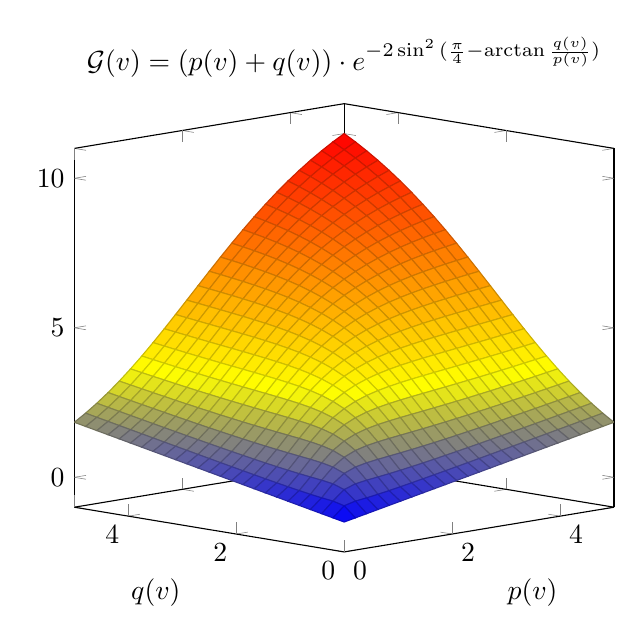
\begin{tikzpicture}[
    declare function={tf(\x)=(pi/4-rad(atan(\x)));},
    declare function={func(\x,\y)=sin(tf(\y/\x)*180/pi);}
]
\begin{axis}[
    view={315}{10},
    title={$
\mathcal{G}(v) = (p(v) + q(v)) \cdot e^{-2\sin^2{(\frac{\pi}{4} -
\arctan\frac{q(v)}{p(v)})}}$},
    xlabel=$p(v)$,
    ylabel=$q(v)$,
]

\addplot3 [
        surf,
        domain=0:5,
        domain y=0:5,
    ] {(x+y)*exp((-2)*(func(x,y))^2)};
\end{axis}
\end{tikzpicture}

	\caption{In-and-out degree curve \label{fig-surf}}
\end{figure}

	\item Computing the Wilbur function with input $G(x,y)$ as the final criterion with respect to the in-and-out degree $\beta$.
\end{enumerate}

\section*{Calculation of AR}
The AR is defined to be the multiplying of the two criteria above, i.e. $\alpha\beta$.


\end{document}
